\documentclass[cs4size,a4paper,10pt]{ctexart}   

\linespread{1.5}
\usepackage{geometry}%用于设置上下左右页边距
	\geometry{left=2.5cm,right=2.5cm,top=3.2cm,bottom=2.7cm}
\usepackage{xeCJK,amsmath,paralist,enumerate,booktabs,multirow,graphicx,subfig,setspace,listings,lastpage,hyperref}
\usepackage{amsthm, amssymb, bm, color, framed, graphicx, hyperref, mathrsfs}
\usepackage{mathrsfs}  
	\setlength{\parindent}{2em}
	\lstset{language=Matlab}%
\usepackage{fancyhdr}
\usepackage{graphicx}
\usepackage{subfloat}
\usepackage{listings}
\usepackage{xcolor}
\usepackage{float}
\usepackage{paralist}
\usepackage{setspace}
\usepackage{titlesec}
\usepackage{enumitem}
\usepackage{hyperref}
\usepackage{multirow}
\usepackage{threeparttable}
\usepackage{autobreak}
\usepackage{multicol}
\usepackage{subfig}
\usepackage{unicode-math}
\usepackage{ltxtable, filecontents}
\usepackage{array}

\hypersetup{
	colorlinks=true,
	linkcolor=black,
	urlcolor=black
}

\setenumerate{partopsep=0pt,topsep=0pt}
\setitemize{itemsep=0pt,partopsep=0pt,topsep=0pt}

\titlespacing*{\section}{0pt}{3pt}{3pt}
\titlespacing*{\subsection}{0pt}{2pt}{2pt}
\titlespacing*{\subsubsection}{0pt}{1pt}{1pt}
\titlespacing*{\paragraph}{0pt}{0pt}{0pt}

\ctexset{secnumdepth=4,tocdepth=4}
\setlength{\parindent}{0pt}
\setstretch{1.2}


\setCJKmainfont[BoldFont={FZHei-B01},ItalicFont={FZKai-Z03}]{FZShuSong-Z01} 
\setCJKsansfont[BoldFont={FZHei-B01}]{FZKai-Z03} 
\setCJKmonofont[BoldFont={FZHei-B01}]{FZFangSong-Z02}
\setCJKfamilyfont{zhsong}{FZShuSong-Z01} 
\setCJKfamilyfont{zhhei}{FZHei-B01} 
\setCJKfamilyfont{zhkai}[BoldFont={FZHei-B01}]{FZKai-Z03} 
\setCJKfamilyfont{zhfs}[BoldFont={FZHei-B01}]{FZFangSong-Z02} 
\renewcommand*{\songti}{\CJKfamily{zhsong}} 
\renewcommand*{\heiti}{\CJKfamily{zhhei}} 
\renewcommand*{\kaishu}{\CJKfamily{zhkai}} 
\renewcommand*{\fangsong}{\CJKfamily{zhfs}}


\definecolor{mKeyword}{RGB}{0,0,255}          % bule
\definecolor{mString}{RGB}{160,32,240}        % purple
\definecolor{mComment}{RGB}{34,139,34}        % green
\definecolor{mNumber}{RGB}{128,128,128} 

\lstdefinestyle {njulisting} {
	basewidth = 0.5 em,
	lineskip = 3 pt,
	basicstyle = \small\ttfamily,
	% keywordstyle = \bfseries,
	commentstyle = \itshape\color{gray}, 
	basicstyle=\small\ttfamily,
	keywordstyle={\color{black}},     % sets color for keywords
	stringstyle={\color{black}},       % sets color for strings
	commentstyle={\color{black}},     % sets color for comments
	numberstyle=\tiny\color{black},
	numbers = left,
	captionpos = t,
	breaklines = true,
	xleftmargin = 1 em,
	xrightmargin = 0 em,
	frame=tlrb,
	tabsize=4,
	aboveskip = 7 pt, %与代码环境上一行的垂直间距
    belowskip = -2 pt %与代码环境下一行的垂直间距
}

\lstset{
style = njulisting, % 调用上述样式 
flexiblecolumns % 允许调整字符宽度
}

\newcommand \sverb {\ \verb}

%================= 基本格式预置 ===========================
\usepackage{fancyhdr}
\pagestyle{fancy}
\lhead{数据管理基础}
\rhead{数据库完整性}
\cfoot{\thepage}
\renewcommand{\headrulewidth}{0.4pt}
\renewcommand{\theenumi}{(\arabic{enumi})}
\CTEXsetup[format={\bfseries\zihao{-3}}]{section}
\CTEXsetup[format={\bfseries\zihao{4}}]{subsection}
\CTEXsetup[format={\bfseries\zihao{-4}}]{subsubsection}


\renewcommand{\contentsname}{目录}  
\begin{document}

	\begin{center}
		{\huge\textbf{第五章\ 数据库完整性}}
	\end{center}
	%---------目录---------% 
	\pagenumbering{Roman}
	\tableofcontents
	\clearpage

 	%---------正文---------% 
	\pagenumbering{arabic}
	\setcounter{page}{1}
	\setlength{\parskip}{0.65em}

	\setlength\abovedisplayskip{5pt}
	\setlength\belowdisplayskip{5pt}

	数据库的完整性是指数据的正确性和相容性
\begin{itemize}
    \item 数据的正确性是指数据是符合现实世界语义,反映了当前实际状况的
    \item 数据的相容性是指数据库同一对象在不同关系表中的数据是符合逻辑的
\end{itemize}

数据的完整性和安全性是两个既有联系又不尽相同的概念
\begin{itemize}
    \item 数据的完整性
    \begin{itemize}
        \item 防止数据库中存在不符合语义的数据,也就是防止数据库中存在不正确的数据
        \item 防范对象:不合语义的、不正确的数据
    \end{itemize}
    \item 数据的安全性
    \begin{itemize}
        \item 保护数据库,防止恶意的破坏和非法的存取
        \item 防范对象:非法用户和非法操作
    \end{itemize}
\end{itemize}

为维护数据库的完整性,数据库管理系统必须实现如下功能
\begin{itemize}
    \item 提供定义完整性约束条件的机制
    \begin{itemize}
        \item 完整性约束条件也称为完整性规则,是数据库中的数据必须满足的语义约束条件
        \item SQL 标准使用了一系列概念来描述完整性,包括关系模型的实体完整性、参照完整性和用户定义完整性
        \item 这些完整性一般由 SQL 的数据定义语言语句来实现 
    \end{itemize}
    \item 提供完整性检查的方法
    \begin{itemize}
        \item 数据库管理系统中检查数据是否满足完整性约束条件的机制称为完整性检查。
        \item 一般在\sverb|INSERT|、\verb|UPDATE|、\verb|DELETE|\ 语句执行后开始检查,也可以在事务提交时检查
    \end{itemize}
    \item 进行违约处理
    \begin{itemize}
        \item 数据库管理系统若发现用户的操作违背了完整性约束条件,就采取一定的动作,如拒绝(NO ACTION)执行该操作或级联(CASCADE)执行其他操作
    \end{itemize}
\end{itemize}
 
\section{实体完整性}

\subsection{定义实体完整性}
关系模型的实体完整性在\sverb|CREATE TABLE|\ 中用\sverb|PRIMARY KEY|\ 定义。单属性构成的码有两种说明方法,一种是定义为列级约束条件,另一种是定义为表级约束条件;对多个属性构成的码只有一种说明方法,即定义为表级约束条件

例:将SC表中的Sno,Cno属性组定义为码
\begin{lstlisting}
CREATE TABLE SC
	(Sno CHAR(9) NOT NULL, 
	Cno CHAR(4) NOT NULL,  
	Grade SMALLINT,
	PRIMARY KEY (Sno,Cno)
	); 
\end{lstlisting}

\subsection{实体完整性检查和违约处理}
插入或对主码列进行更新操作时,关系数据库管理系统按照实体完整性规则自动进行检查。包括:
\begin{itemize}
    \item 检查主码值是否唯一,如果不唯一则拒绝插入或修改
    \item 检查主码的各个属性是否为空,只要有一个为空就拒绝插入或修改
\end{itemize}

\section{参照完整性}

\subsection{定义参照完整性}
关系模型的参照完整性在\sverb|CREATE TABLE|\ 中用\sverb|FOREIGN KEY|\ 短语定义哪些列为外码,用 \sverb|REFERENCES|\ 短语指明这些外码参照哪些表的主码

例:关系SC中一个元组表示一个学生选修的某门课程的成绩,(Sno,Cno)是主码。Sno、Cno分别参照引用Student表的主码和Course表的主码。定义SC中的参照完整性
\begin{lstlisting}
CREATE TABLE SC
	(Sno CHAR(9) NOT NULL, 
	Cno CHAR(4) NOT NULL,  
	Grade SMALLINT,
	PRIMARY KEY (Sno, Cno),  
	FOREIGN KEY (Sno) REFERENCES Student(Sno),  
	FOREIGN KEY (Cno) REFERENCES Course(Cno)    
	);
\end{lstlisting}

\subsection{参照完整性检查和违约处理}
可能破坏参照完整性的情况及违约处理
\begin{figure}[H]
    \vspace{-0.5em}
	\centering
	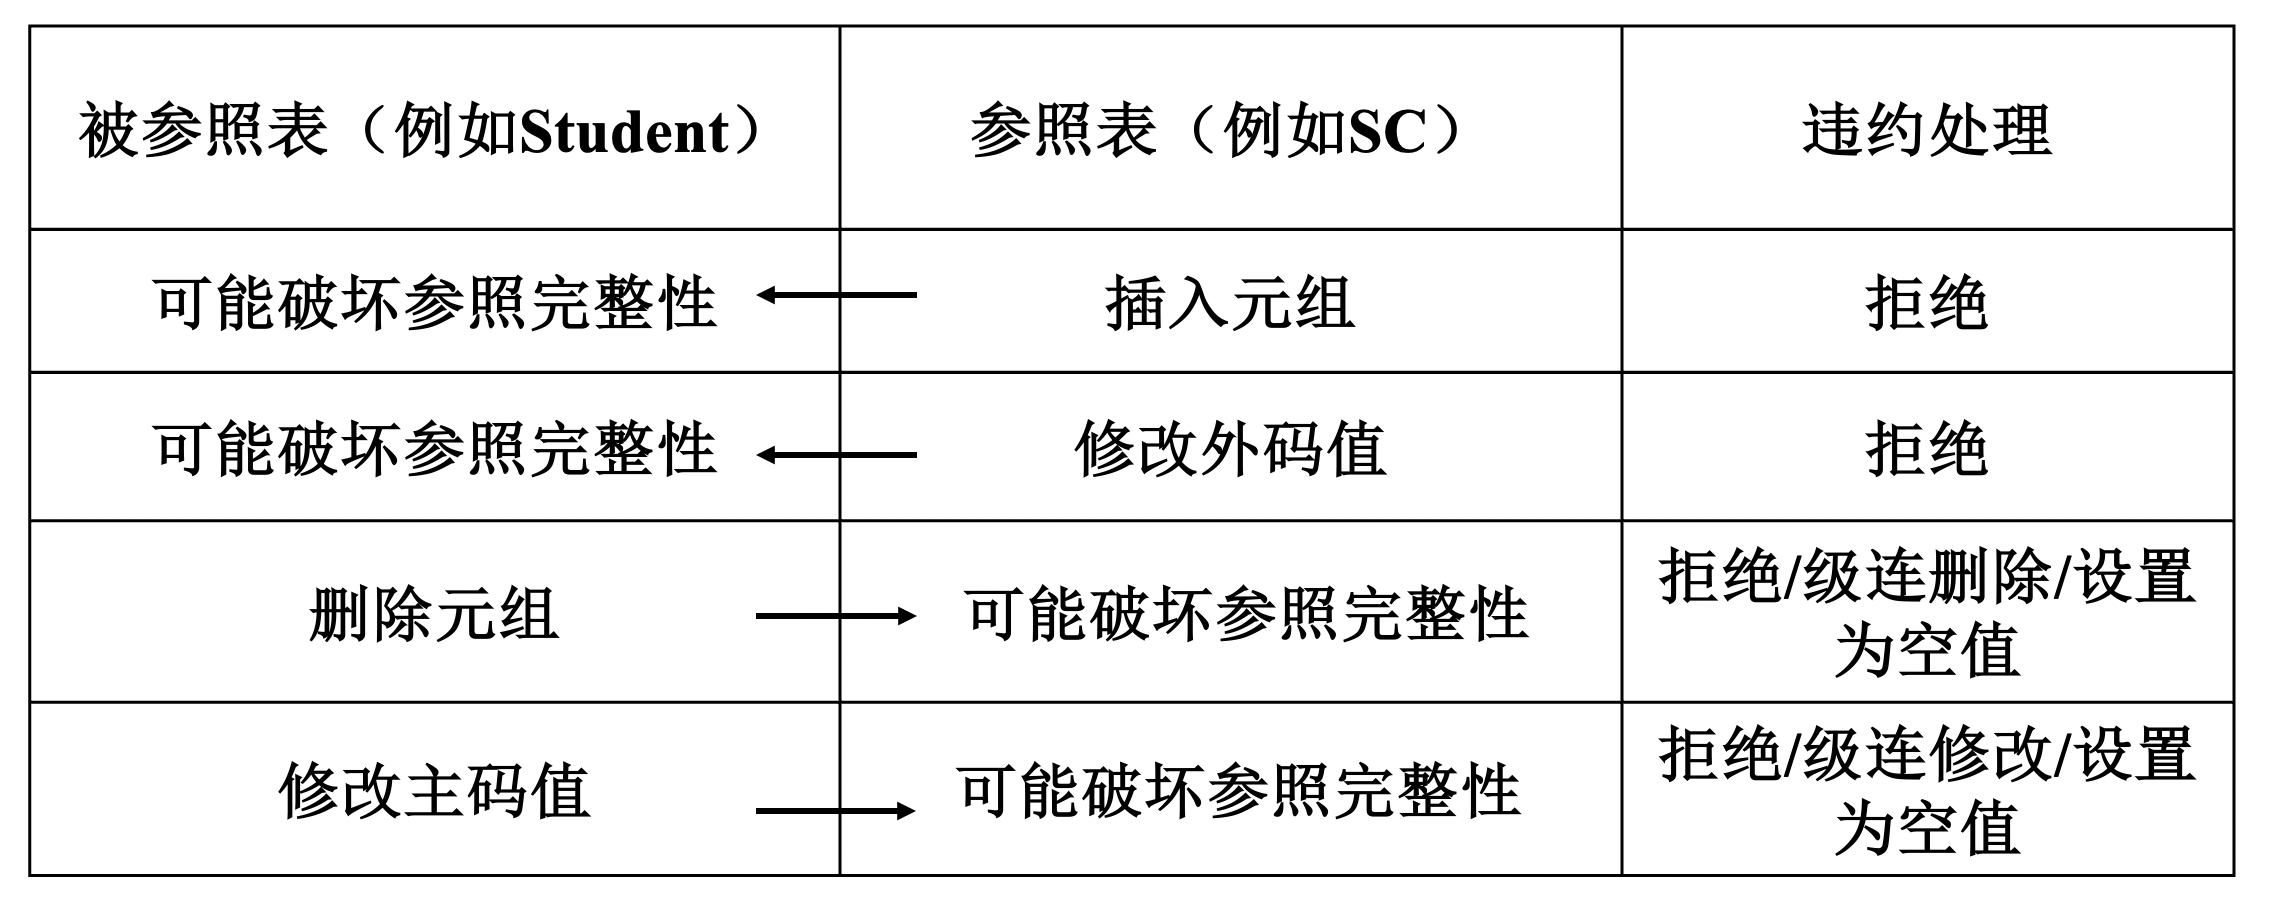
\includegraphics[width=0.65\textwidth]{images/5.2.2}
    \vspace{-1em}
\end{figure}

例:显式说明参照完整性的违约处理示例
\begin{lstlisting}
CREATE TABLE SC
(Sno CHAR(9) NOT NULL,
Cno CHAR(4) NOT NULL,
Grade SMALLINT,
PRIMARY KEY(Sno,Cno), 			
FOREIGN KEY (Sno) REFERENCES Student(Sno) /* 在表级定义参照完整性 */
	ON DELETE CASCADE   /* 当删除Student表中的元组时,级联删除SC表中相应的元组 */
	ON UPDATE CASCADE,  /* 当更新Student表中的sno时,级联更新SC表中相应的元组 */
FOREIGN KEY (Cno) REFERENCES Course(Cno)  /* 在表级定义参照完整性 */                    
	ON DELETE NO ACTION /* 当删除Course表中的元组造成了与SC表不一致时,拒绝删除 */
	ON UPDATE CASCADE   /* 当更新Course表中的Cno时,级联更新SC表中相应的元组 */
);
\end{lstlisting}

\section{用户定义的完整性}

\subsection{属性上的约束条件}

\subsubsection{属性上约束条件的定义}
在\sverb|CREATE TABLE|\ 中定义属性的同时,可以根据应用要求定义属性上的约束条件,即属性值限制,包括
\begin{itemize}
    \item 列值非空(\verb|NOT NULL|)
    \item 列值唯一(\verb|UNIQUE|)
    \item 检查列值是否满足一个条件表达式(\verb|CHECK|\ 短语)
\end{itemize}

例:Student表的Ssex只允许取“男”或“女”
\begin{lstlisting}
CREATE TABLE Student
	(Sno CHAR(9) PRIMARY KEY,
	Sname CHAR(8) NOT NULL,                     
	Ssex CHAR(2) CHECK (Ssex IN ('男','女')),           
	Sage SMALLINT,
	Sdept CHAR(20)
);
\end{lstlisting}

\subsubsection{属性上约束条件的检查和违规处理}
当往表中插入元组或修改属性的值时,关系数据库管理系统将检查属性上的约束条件是否被满足,如果不满足则操作被拒绝执行

\subsection{元组上的约束条件}

\subsubsection{元组上约束条件的定义}
元组级的限制可以设置不同属性之间的取值的相互约束条件

例:当学生的性别是男时,其名字不能以Ms.打头
\begin{lstlisting}
CREATE TABLE Student
	(Sno CHAR(9), 
	Sname CHAR(8) NOT NULL,
	Ssex CHAR(2),
	Sage SMALLINT,
	Sdept CHAR(20),
	PRIMARY KEY (Sno),
	CHECK (Ssex = '女' OR Sname NOT LIKE 'Ms.%')
);
\end{lstlisting}

\subsubsection{元组上约束条件的检查和违约处理}
当往表中插入元组或修改属性的值时,关系数据库管理系统将检查元组上的约束条件是否被满足,如果不满足则操作被拒绝执行

\section{完整性约束命名子句}

\subsection{完整性约束命名子句}
\begin{lstlisting}
CONSTRAINT <完整性约束条件名><完整性约束条件>
\end{lstlisting}
\verb|<完整性约束条件>|\ 包括\sverb|NOT NULL|、\verb|UNIQUE|、\verb|PRIMARY KEY|\ 短语、\verb|FOREIGN KEY|\ 短语、\verb|CHECK|\ 短语等

\subsection{修改表中的完整性限制}
使用\sverb|ALTER TABLE|\ 语句修改表中的完整性限制

例:修改表Student中的约束条件,要求学号改为在$900000\sim 999999$之间,年龄由小于30改为小于40
\begin{lstlisting}
/*可以先删除原来的约束条件,再增加新的约束条件*/
ALTER TABLE Student
	DROP CONSTRAINT C1;
ALTER TABLE Student
	ADD CONSTRAINT C1 CHECK (Sno BETWEEN 900000 AND 999999),
ALTER TABLE Student
	DROP CONSTRAINT C3;
ALTER TABLE Student
	ADD CONSTRAINT C3 CHECK(Sage < 40);
\end{lstlisting}

\section{断言}
\begin{itemize}
    \item SQL 中,可以使用\sverb|CREATE ASSERTION|\ 语句,通过声明性断言来指定更具一般性的约束
    \item 可以定义涉及多个表的或聚集操作的比较复杂的完整性约束
    \item 断言创建以后,任何对断言中所涉及的关系的操作都会触发关系数据库管理系统对断言的检查,任何使断言不为真值的操作都会被拒绝执行
\end{itemize}

\subsection{创建断言的语句格式}
\begin{lstlisting}
CREATE ASSERTION <断言名> <CHECK 子句>
\end{lstlisting}

每个断言都被赋予一个名字,\verb|<CHECK 子句>|\ 中的约束条件与\verb|WHERE|\ 子句的条件表达式类似

例:限制数据库课程最多60名学生选修
\begin{lstlisting}
CREATE ASSERTION ASSE_SC_DB_NUM
    CHECK (60 >= (SELECT COUNT(*)
        FROM Course,SC
        WHERE SC.Cno = Course.Cno AND Course.Cname = '数据库')
    );
\end{lstlisting}

\subsection{删除断言的语句格式} 
\begin{lstlisting}
DROP ASSERTION <断言名>;
\end{lstlisting}

\section{触发器}
\begin{itemize}
    \item 触发器是用户定义在关系表上的一类由事件驱动的特殊过程
    \begin{itemize}
        \item 触发器保存在数据库服务器中
        \item 任何用户对表的增、删、改操作均由服务器自动激活相应的触发器
        \item 触发器可以实施更为复杂的检查和操作,具有更精细和更强大的数据控制能力
    \end{itemize}
    \item 不同的关系数据库管理系统触发器语法各不相同
\end{itemize}

\subsection{定义触发器}
\begin{lstlisting}
CREATE TRIGGER <触发器名>  
{BEFORE | AFTER} <触发事件> ON <表名>
REFERENCING NEW | OLD ROW AS<变量>
FOR EACH  {ROW | STATEMENT}
[WHEN <触发条件>]<触发动作体>
\end{lstlisting}

\begin{itemize}
    \item 触发器又叫做事件—条件—动作规则
    \begin{itemize}
        \item 当特定的系统事件发生时,对规则的条件进行检查,如果条件成立则执行规则中的动作,否则不执行该动作。规则中的动作体可以很复杂,通常是一段 SQL 存储过程
    \end{itemize}
    \item 表的拥有者才可以在表上创建触发器
    \item 触发器名
    \begin{itemize}
        \item 触发器名可以包含模式名,也可以不包含模式名
        \item 同一模式下,触发器名必须是唯一的
        \item 触发器名和表名必须在同一模式下
    \end{itemize}
    \item 表名
    \begin{itemize}
        \item 触发器只能定义在基本表上,不能定义在视图上
        \item 当基本表的数据发生变化时,将激活定义在该表上相应触发事件的触发器
    \end{itemize}
    \item 触发事件
    \begin{itemize}
        \item 触发事件可以是\sverb|INSERT|、\verb|DELETE|\ 或\sverb|UPDATE|,也可以是这几个事件的组合
    \end{itemize}
    \item 还可以\sverb|UPDATE OF<触发列,...>|,即进一步指明修改哪些列时激活触发器
    \begin{itemize}
        \item \verb|AFTER/BEFORE|\ 是触发的时机
        \begin{itemize}
            \item \verb|AFTER|\ 表示在触发事件的操作执行之后激活触发器
            \item \verb|BEFORE|\ 表示在触发事件的操作执行之前激活触发器
        \end{itemize}
    \end{itemize}
    \item 触发器类型
    \begin{itemize}
        \item 行级触发器(\verb|FOR EACH ROW|)
        \item 语句级触发器(\verb|FOR EACH STATEMENT|) 
    \end{itemize}
    \item 触发条件
    \begin{itemize}
        \item 触发器被激活时,只有当触发条件为真时触发动作体才执行;否则触发动作体不执行。
        \item 如果省略\sverb|WHEN|\ 触发条件,则触发动作体在触发器激活后立即执行
    \end{itemize}
    \item 触发动作体
    \begin{itemize}
        \item 触发动作体可以是一个匿名 PL/SQL 过程块,也可以是对已创建存储过程的调用
    \end{itemize}
    \item 如果是行级触发器,用户都可以在过程体中使用\sverb|NEW|\ 和\sverb|OLD|\ 引用事件之后的新值和事件之前的旧值
    \begin{itemize}
        \item 如果是语句级触发器,则不能在触发动作体中使用\sverb|NEW|\ 和\sverb|OLD|\ 进行引用
    \end{itemize}
    \item 如果触发动作体执行失败,激活触发器的事件就会终止执行,触发器的目标表或触发器可能影响的其他对象不发生任何变化
\end{itemize}

例:当对表SC的Grade属性进行修改时,若分数增加了10\%则将此次操作记录到下面表中:\verb|SC_U(Sno,|
\verb|Cno, Oldgrade, Newgrade)|\ 其中\sverb|Oldgrade|\ 是修改前的分数,\verb|Newgrade|\ 是修改后的分数
\begin{lstlisting}
CREATE TRIGGER  SC_T		     /* SC_T是触发器的名字 */
AFTER UPDATE OF Grade ON SC  /* UPDATE OF Grade ON SC是触发事件 */
                             /* AFTER是触发时机,表示当对SC的Grade属性修改完后再触发下面的规则 */
REFERENCING
    OLD row AS OldTuple,
    NEW row AS NewTuple
FOR EACH ROW    /* 行级触发器,即每执行一次Grade的更新,下面的规则就执行一次 */
WHEN (NewTuple.Grade >= 1.1 * OldTuple.Grade)       /* 触发条件,只有该条件为真时才执行 */
    INSERT INTO SC_U(Sno, Cno, OldGrade, NewGrade)  /* 下面的INSERT操作 */
    VALUES(OldTuple.Sno, OldTuple.Cno, OldTuple.Grade, NewTuple.Grade) 
\end{lstlisting}

\subsection{激活触发器}
\begin{itemize}
    \item 触发器的执行,是由触发事件激活的,并由数据库服务器自动执行
    \item 一个数据表上可能定义了多个触发器,遵循如下的执行顺序:
    \begin{itemize}
        \item 执行该表上的\sverb|BEFORE|\ 触发器
        \item 激活触发器的 SQL 语句
        \item 执行该表上的\sverb|AFTER|\ 触发器
    \end{itemize}
\end{itemize}

\subsection{删除触发器}
\begin{lstlisting}
DROP TRIGGER <触发器名> ON <表名>; 
\end{lstlisting}




	
	% \begin{figure}[H]
    % \vspace{-0.5em}
	% \centering
	% \includegraphics[width=0.4\textwidth]{images/}
    % \vspace{-1em}
	% \end{figure}

	% \vspace{-0.8em}
	% \begin{multicols}{2}
    % \begin{itemize}
    %     \item 
    % \end{itemize}
	% \end{multicols}
	% \vspace{-1em}


\end{document}


